\documentclass{article}
\usepackage{graphicx}
\usepackage{float}
\usepackage{subcaption}

\begin{document}
\title{Study of two Raspberry Pis and Power adapters}
\author{Abhinav Narain}
\maketitle
\section{Raspberry Pi and Power Adapters}
Two raspberry pis and two adapters and two different adapters were
used for measuring EMI on channel and differences are documented.

\begin{enumerate}
\item Raspberry Pi Model B $+$ V1.2 (Fig~\ref{fig:r1})
\item Raspberry Pi 3 Model BV1.2 (Fig~\ref{fig:r2})
\end{enumerate}

\begin{enumerate}
\item Adapter 1 (Fig ~\ref{fig:p1}) using a USB cable
\item Adapter 2 (Fig ~\ref{fig:p2}) usual usual cable (non-USB) 
\end{enumerate}

\subsection{Compare EMI of two power adapters}
Figure~\ref{fig:u2} shows that the two adapters have distinct EMI on
the channel. The two Raspberry Pis show same signature when one use
the same adapter, showing not much of difference in the two versions
released.

\begin{figure}[H]
  \centering
  \begin{subfigure}{\textwidth}
    \centering
    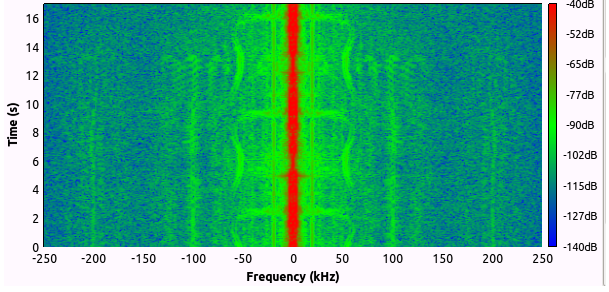
\includegraphics[width=\textwidth]{./figures/raspi-with-usb.png}
    \vspace{-25pt}
    \caption{EMI generated by Raspberry Pi with USB power chord (1)}
    \label{fig:u0}
  \end{subfigure}
  \begin{subfigure}{\textwidth}
    \centering
    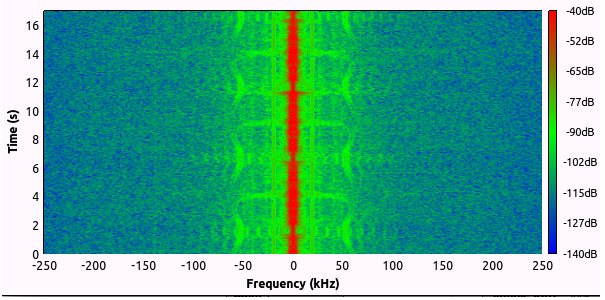
\includegraphics[width=\textwidth]{./figures/raspi-without-usb.png}
    \caption{EMI generated by Raspberry Pi with different power-chord (2)}
    \label{fig:u1}
  \end{subfigure}
  \caption{Same Raspberry Pi-2 shows two different EMI signatures for two different power-chords}
  \label{fig:u2}
\end{figure}

\if0
self comment: This is not correct as the frequency range in second is way more and hence the spectrograms look different.
both of pis produce same EMI on checking later again with experiments.
\subsection{Compare EMI of two Raspberry Pis}
\begin{figure}[H]
  \centering
  \begin{subfigure}{\textwidth}
    \centering
    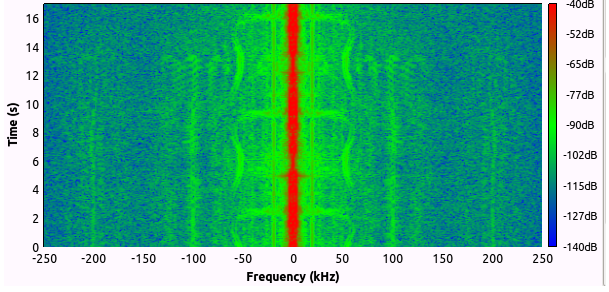
\includegraphics[width=\textwidth]{./figures/raspi-with-usb.png}
    \vspace{-25pt}
    \caption{EMI generated by Raspberry 2 with USB power chord (1)}
    \label{fig:g0}
  \end{subfigure}
  
    \begin{subfigure}{\textwidth}
      \centering
      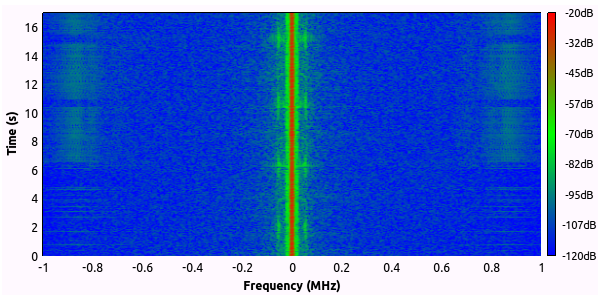
\includegraphics[width=\textwidth]{./figures/raspi-old.png}
      \caption{EMI generated by Raspberry 1 with USB power chord (1)}
      \label{fig:g1}
    \end{subfigure}
    \caption{Two different Raspberry Pi using the same power chord but have different EMI signatures }
    \label{fig:g2}
\end{figure}
\fi
\section{Miscellaneous}
The Raspberry Pis are shown below
\begin{figure*}[t]
  \centering
  \begin{subfigure}{.5\textwidth}
  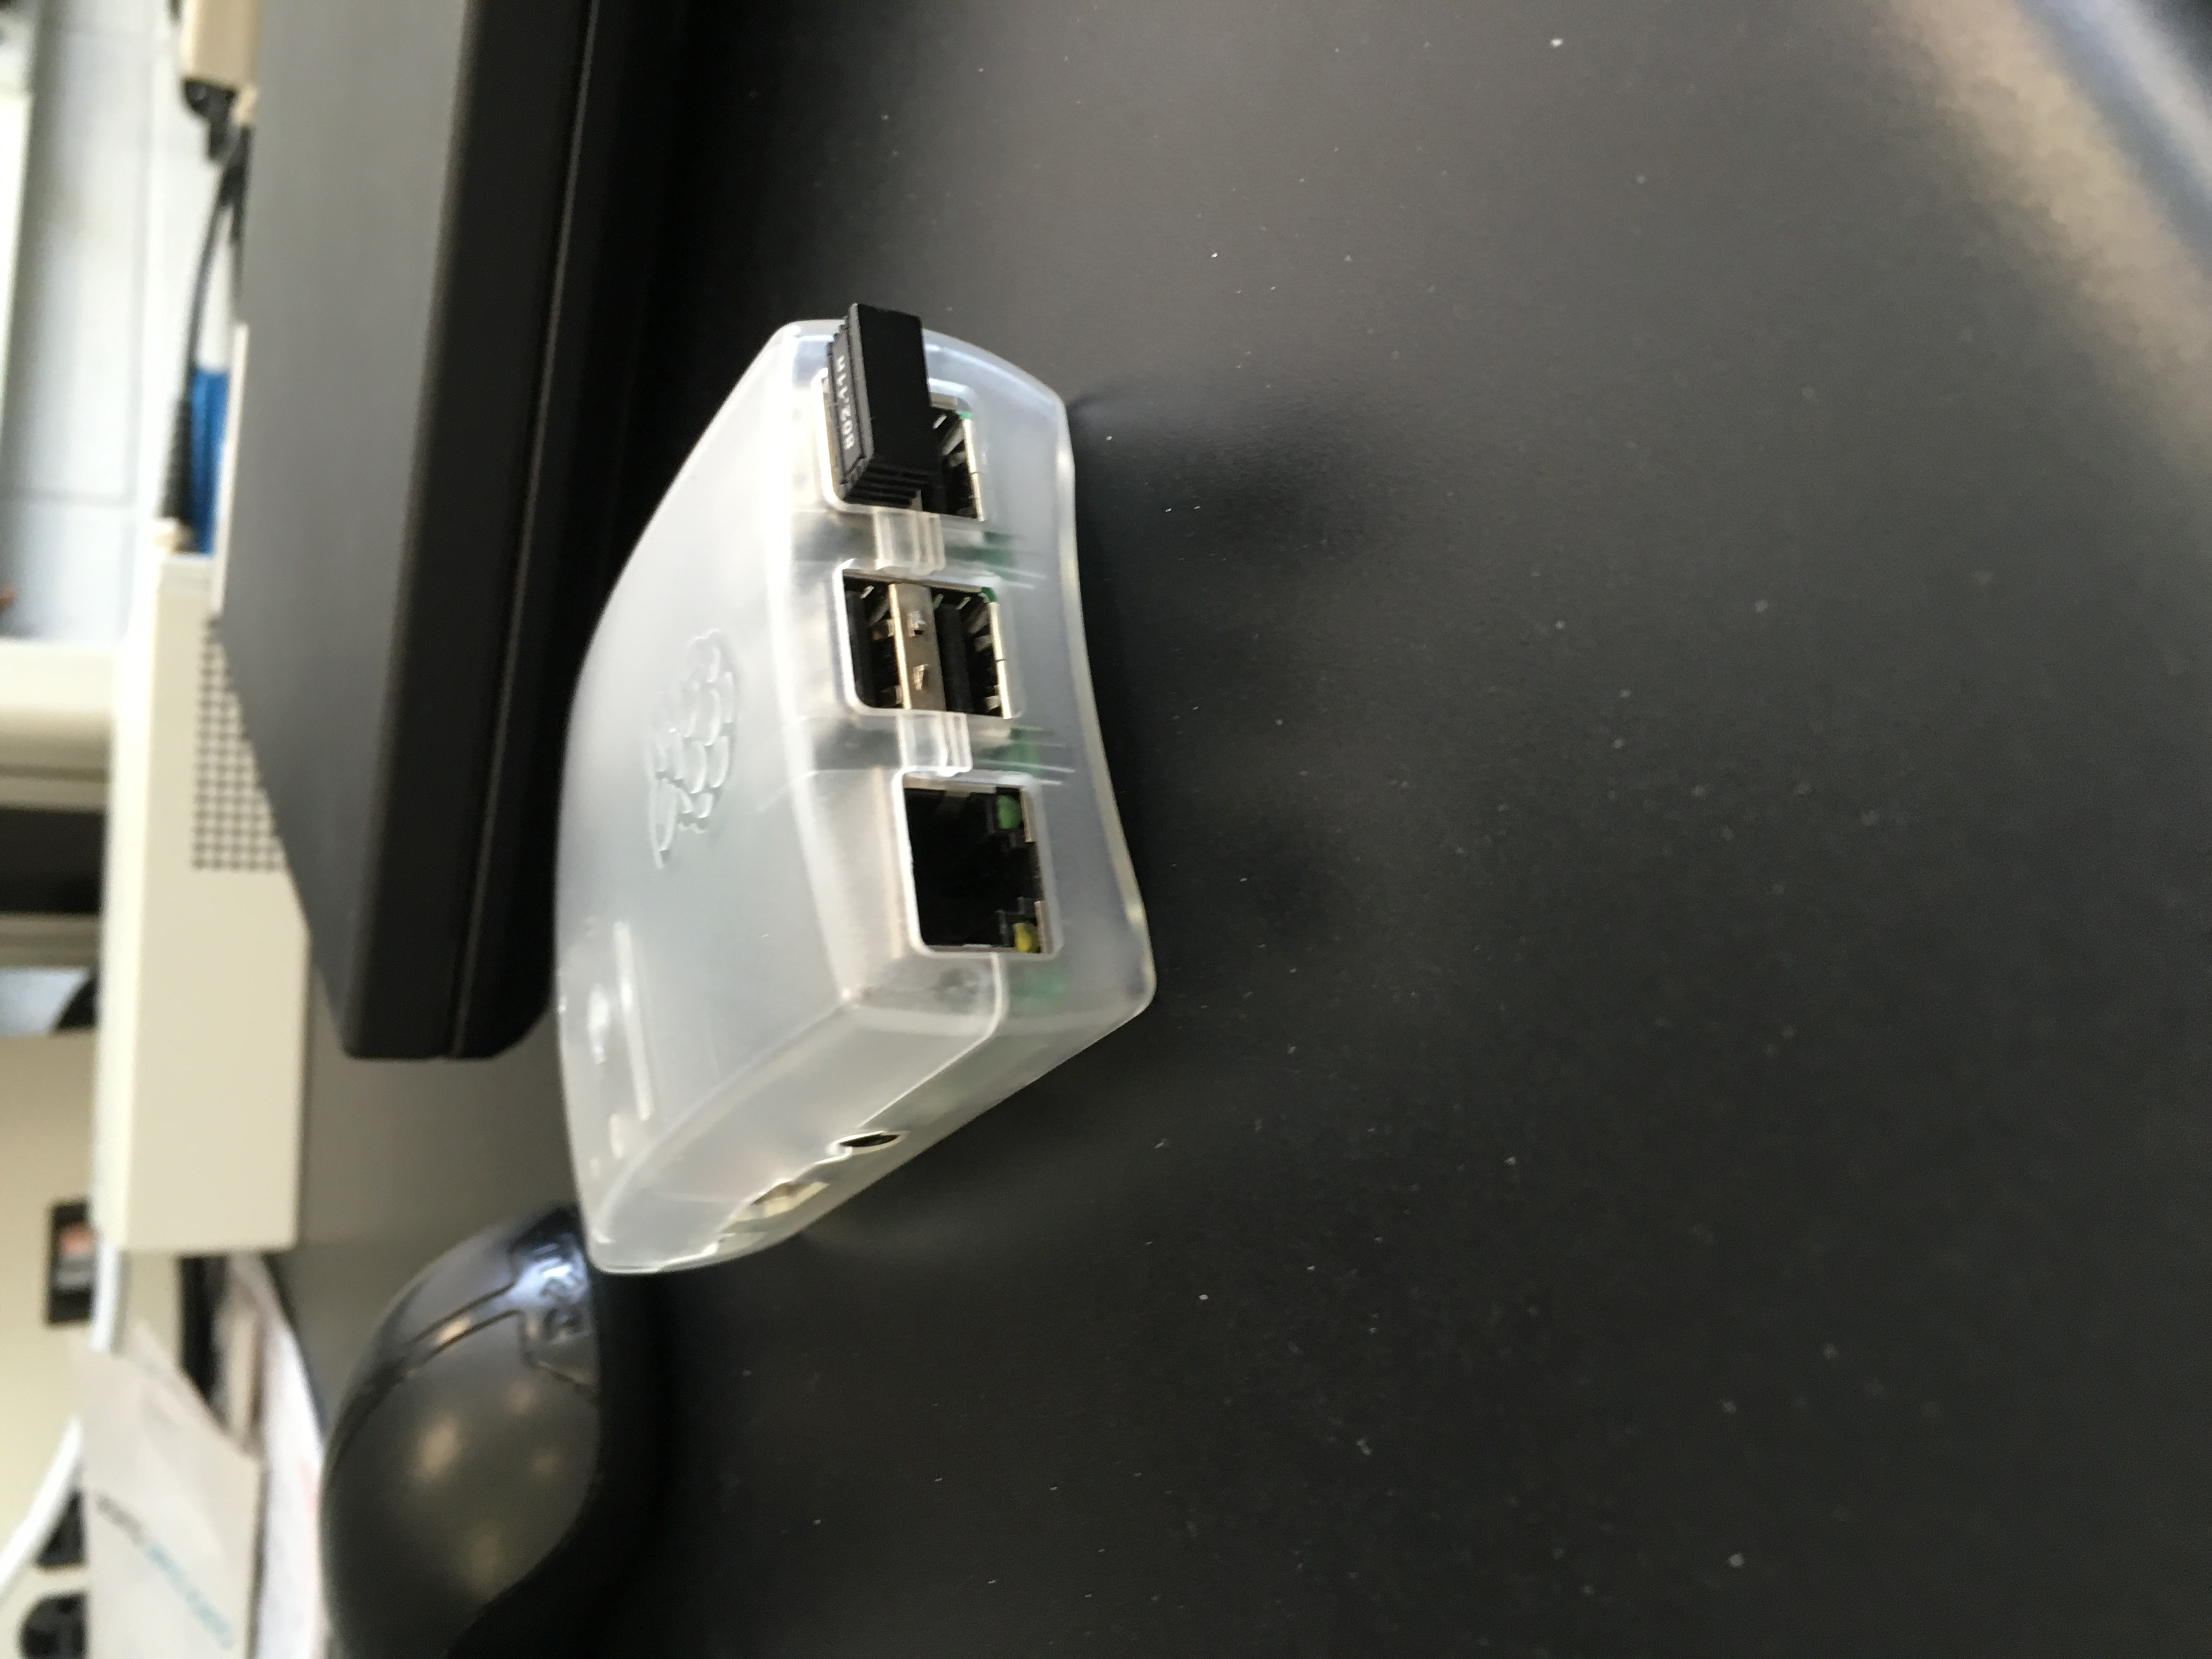
\includegraphics[width=\textwidth]{./figures//IMG_0709.JPG}
  \caption{Raspberry 1 (Raspberry Pi) }
  \label{fig:r1}
  \end{subfigure}\hfill% 
  \centering
  \begin{subfigure}{.5\textwidth}
    \centering
    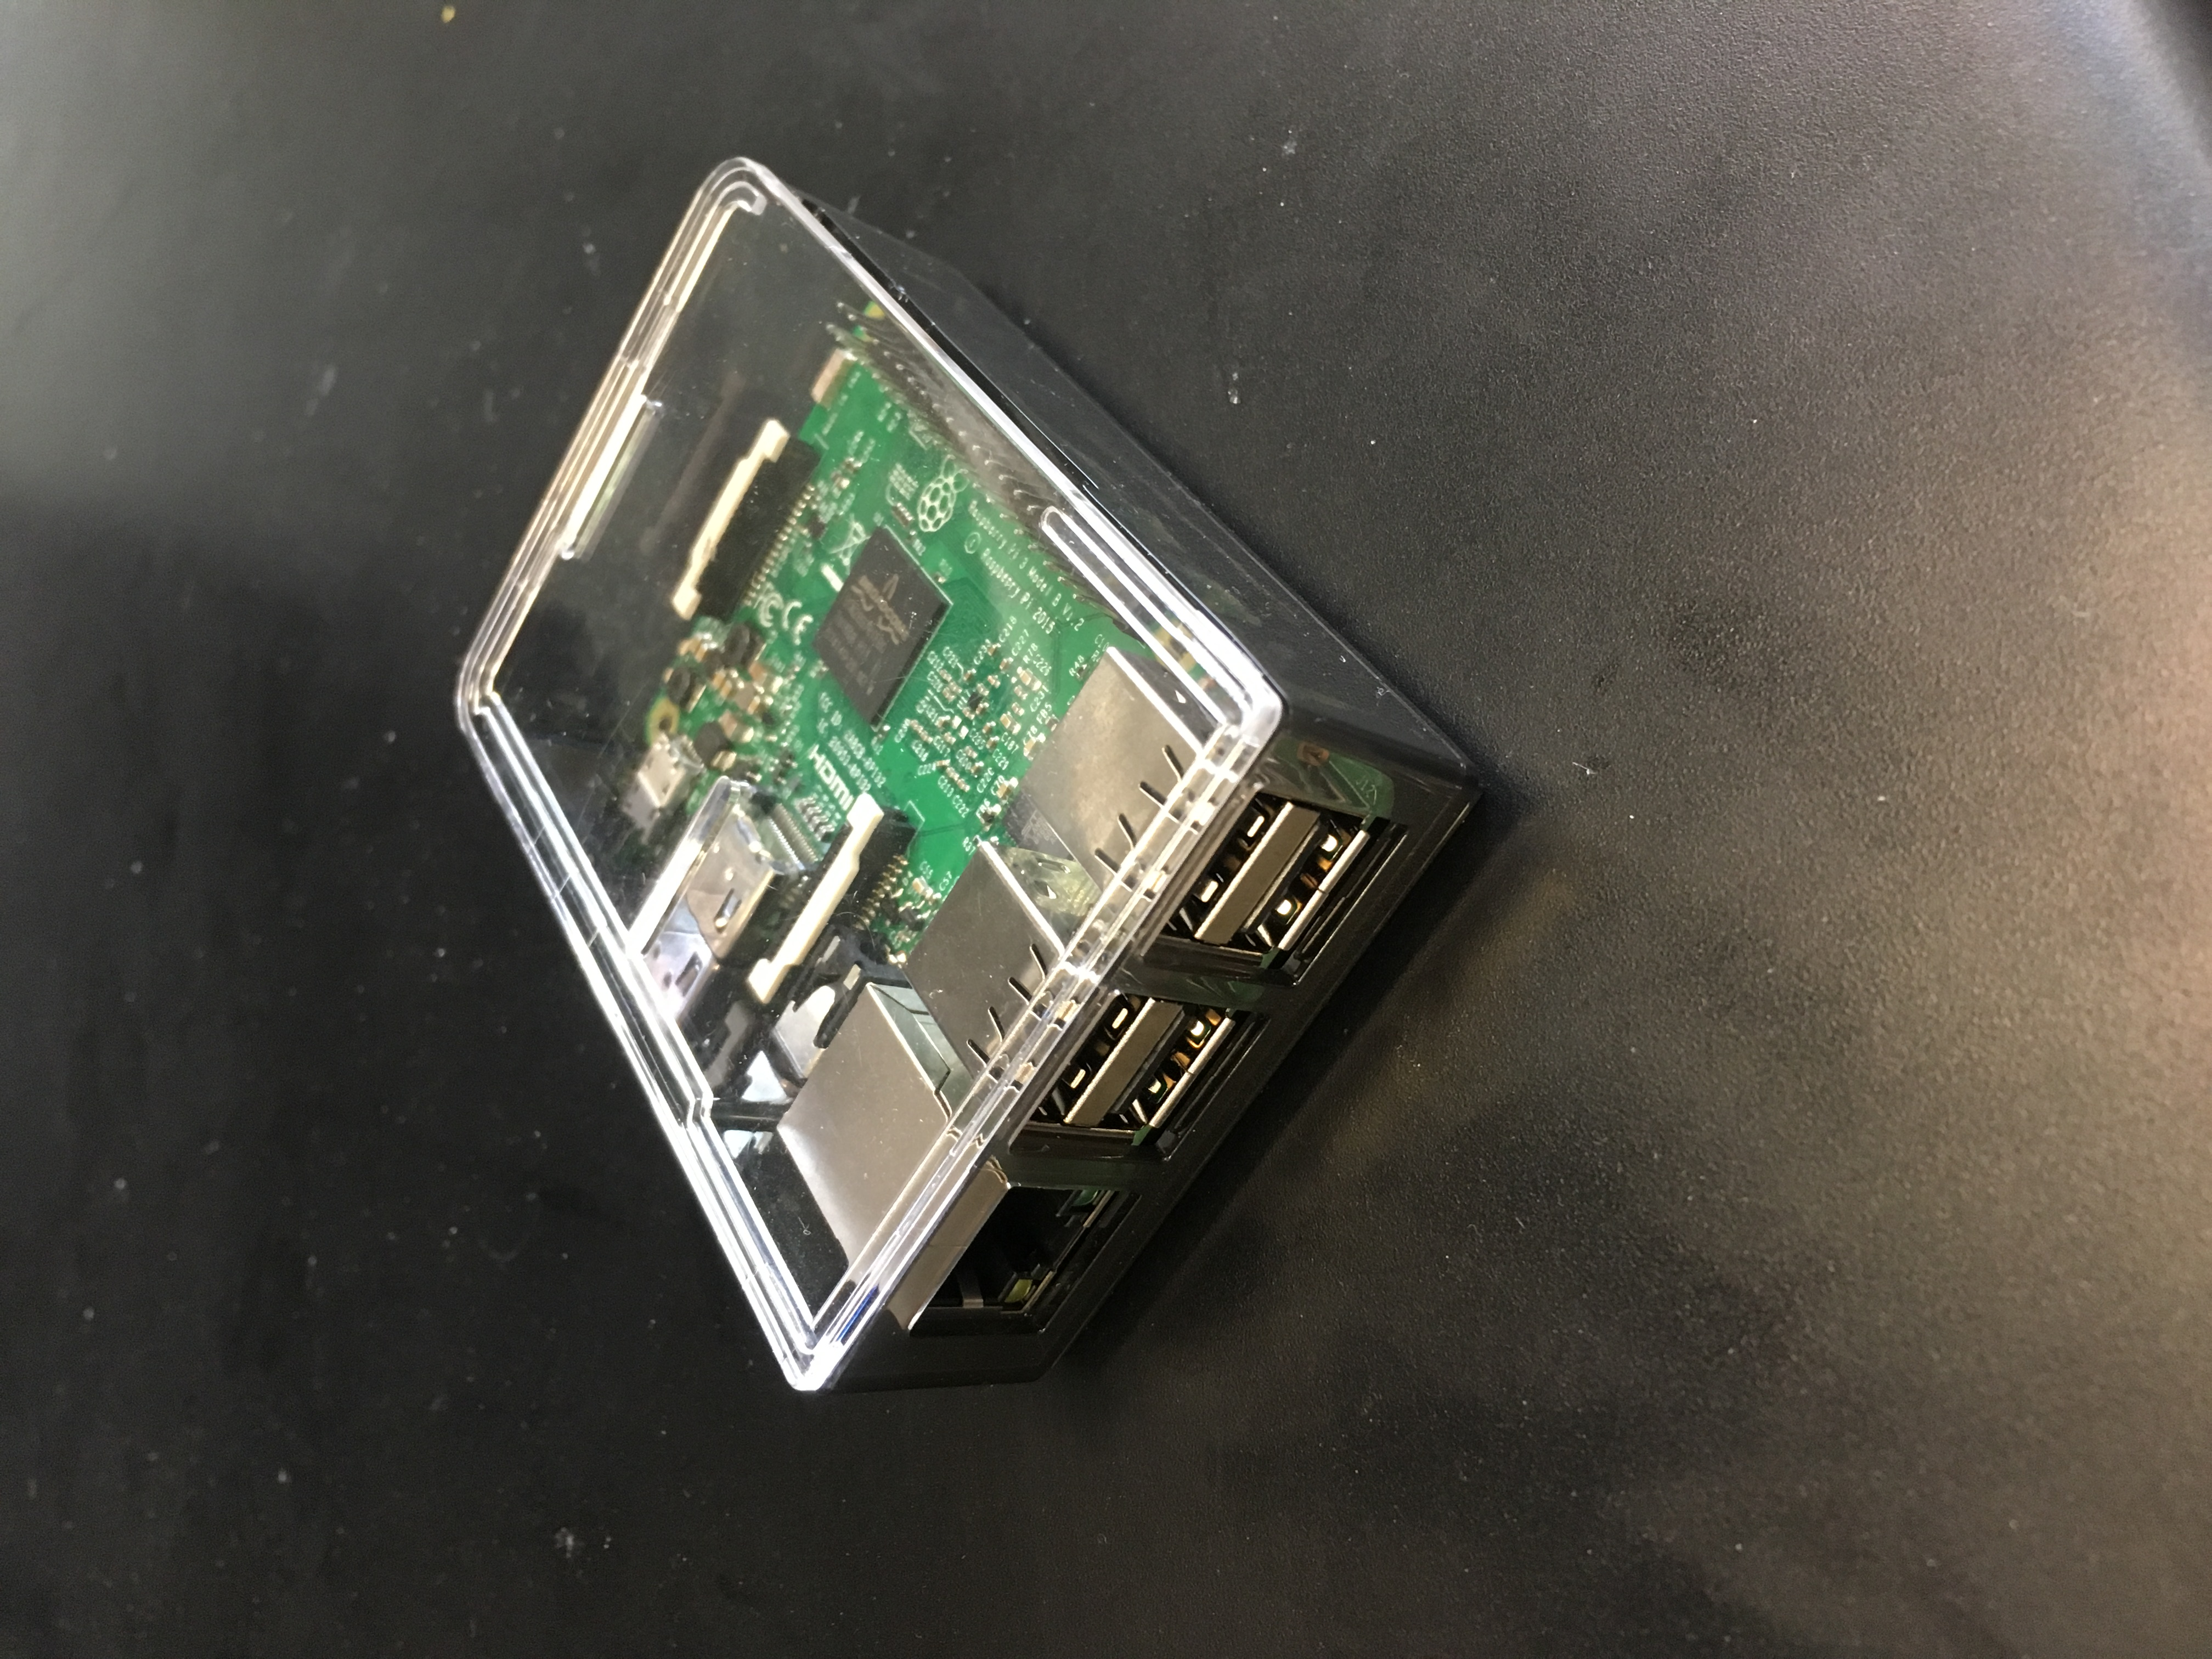
\includegraphics[width=\textwidth]{./figures//IMG_0708.JPG}
    \caption{Raspberry 2 (Raspberry Pi 3)}
    \label{fig:r2}
  \end{subfigure}
  \label{fig:rr}
\end{figure*}

The Adapters are displayed below, first one showing a USB socket and
the second one with usual chord.

\begin{figure*}[t]
  \centering
  \begin{subfigure}{.5\textwidth}
    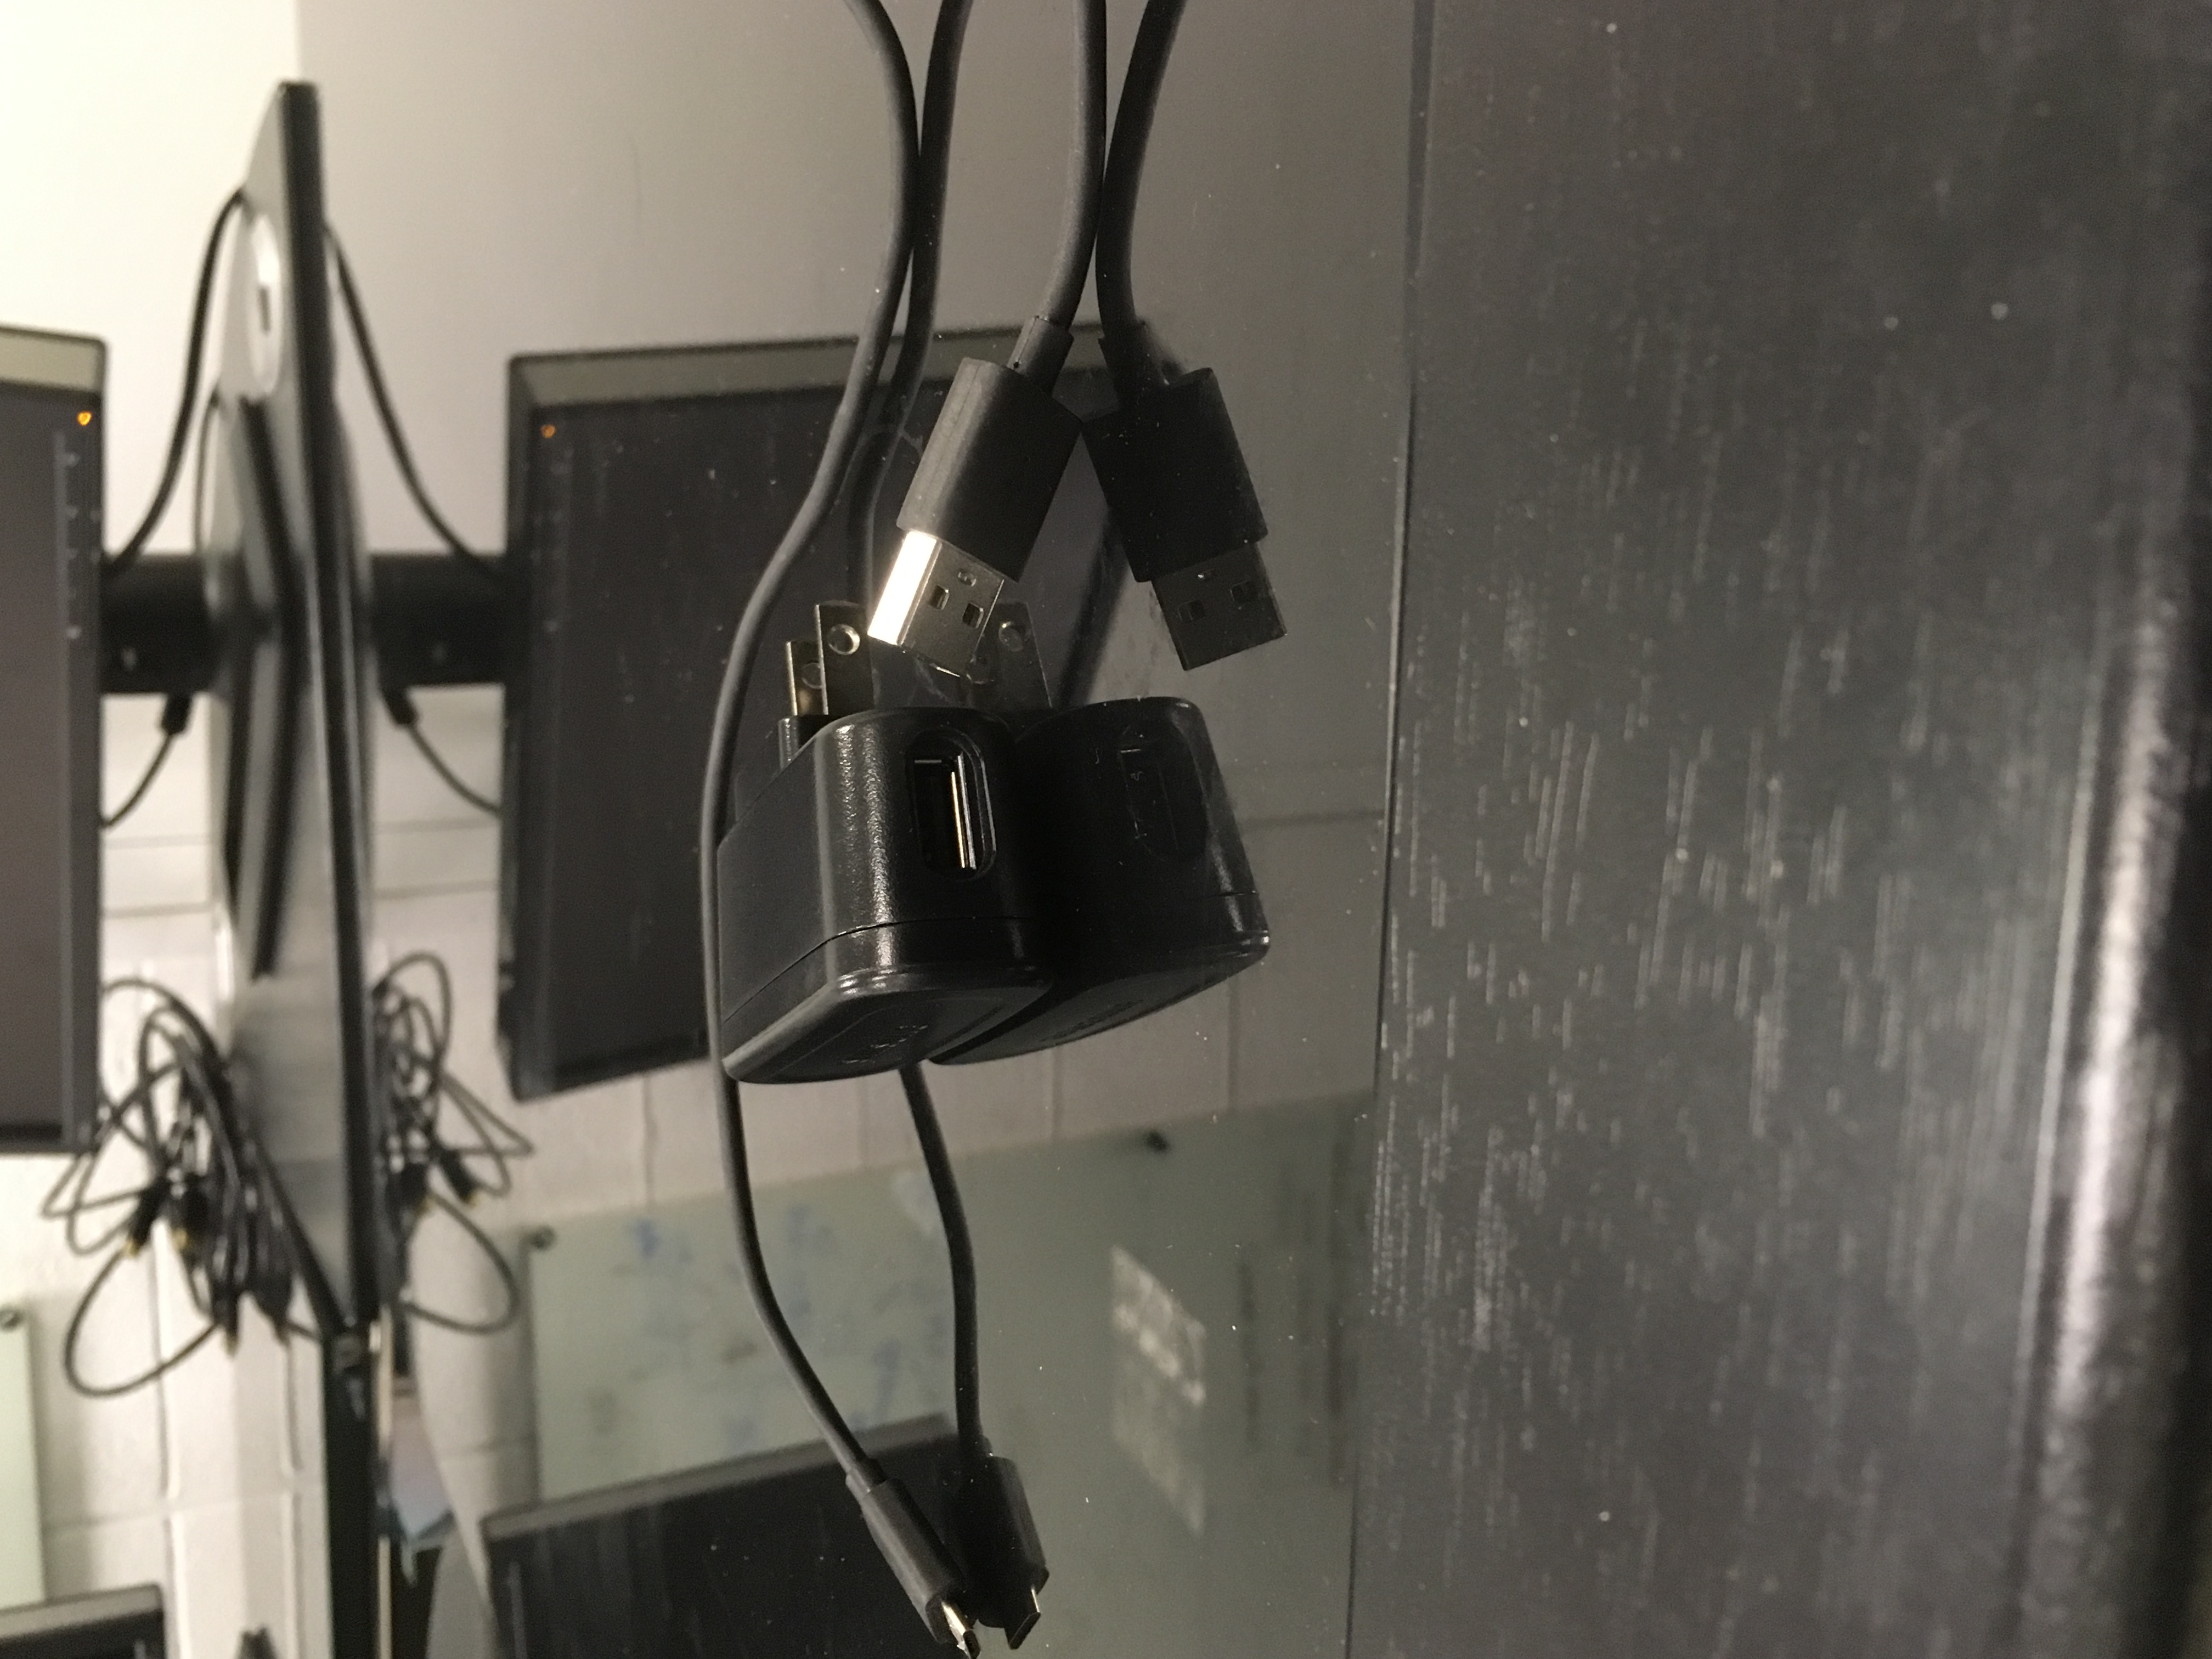
\includegraphics[angle=-90,width=\textwidth]{./figures//IMG_0712.JPG}
    \caption{Adapter 1}
    \label{fig:p1}
  \end{subfigure}\hfill% 
  \centering
  \begin{subfigure}{.5\textwidth}
    \centering
    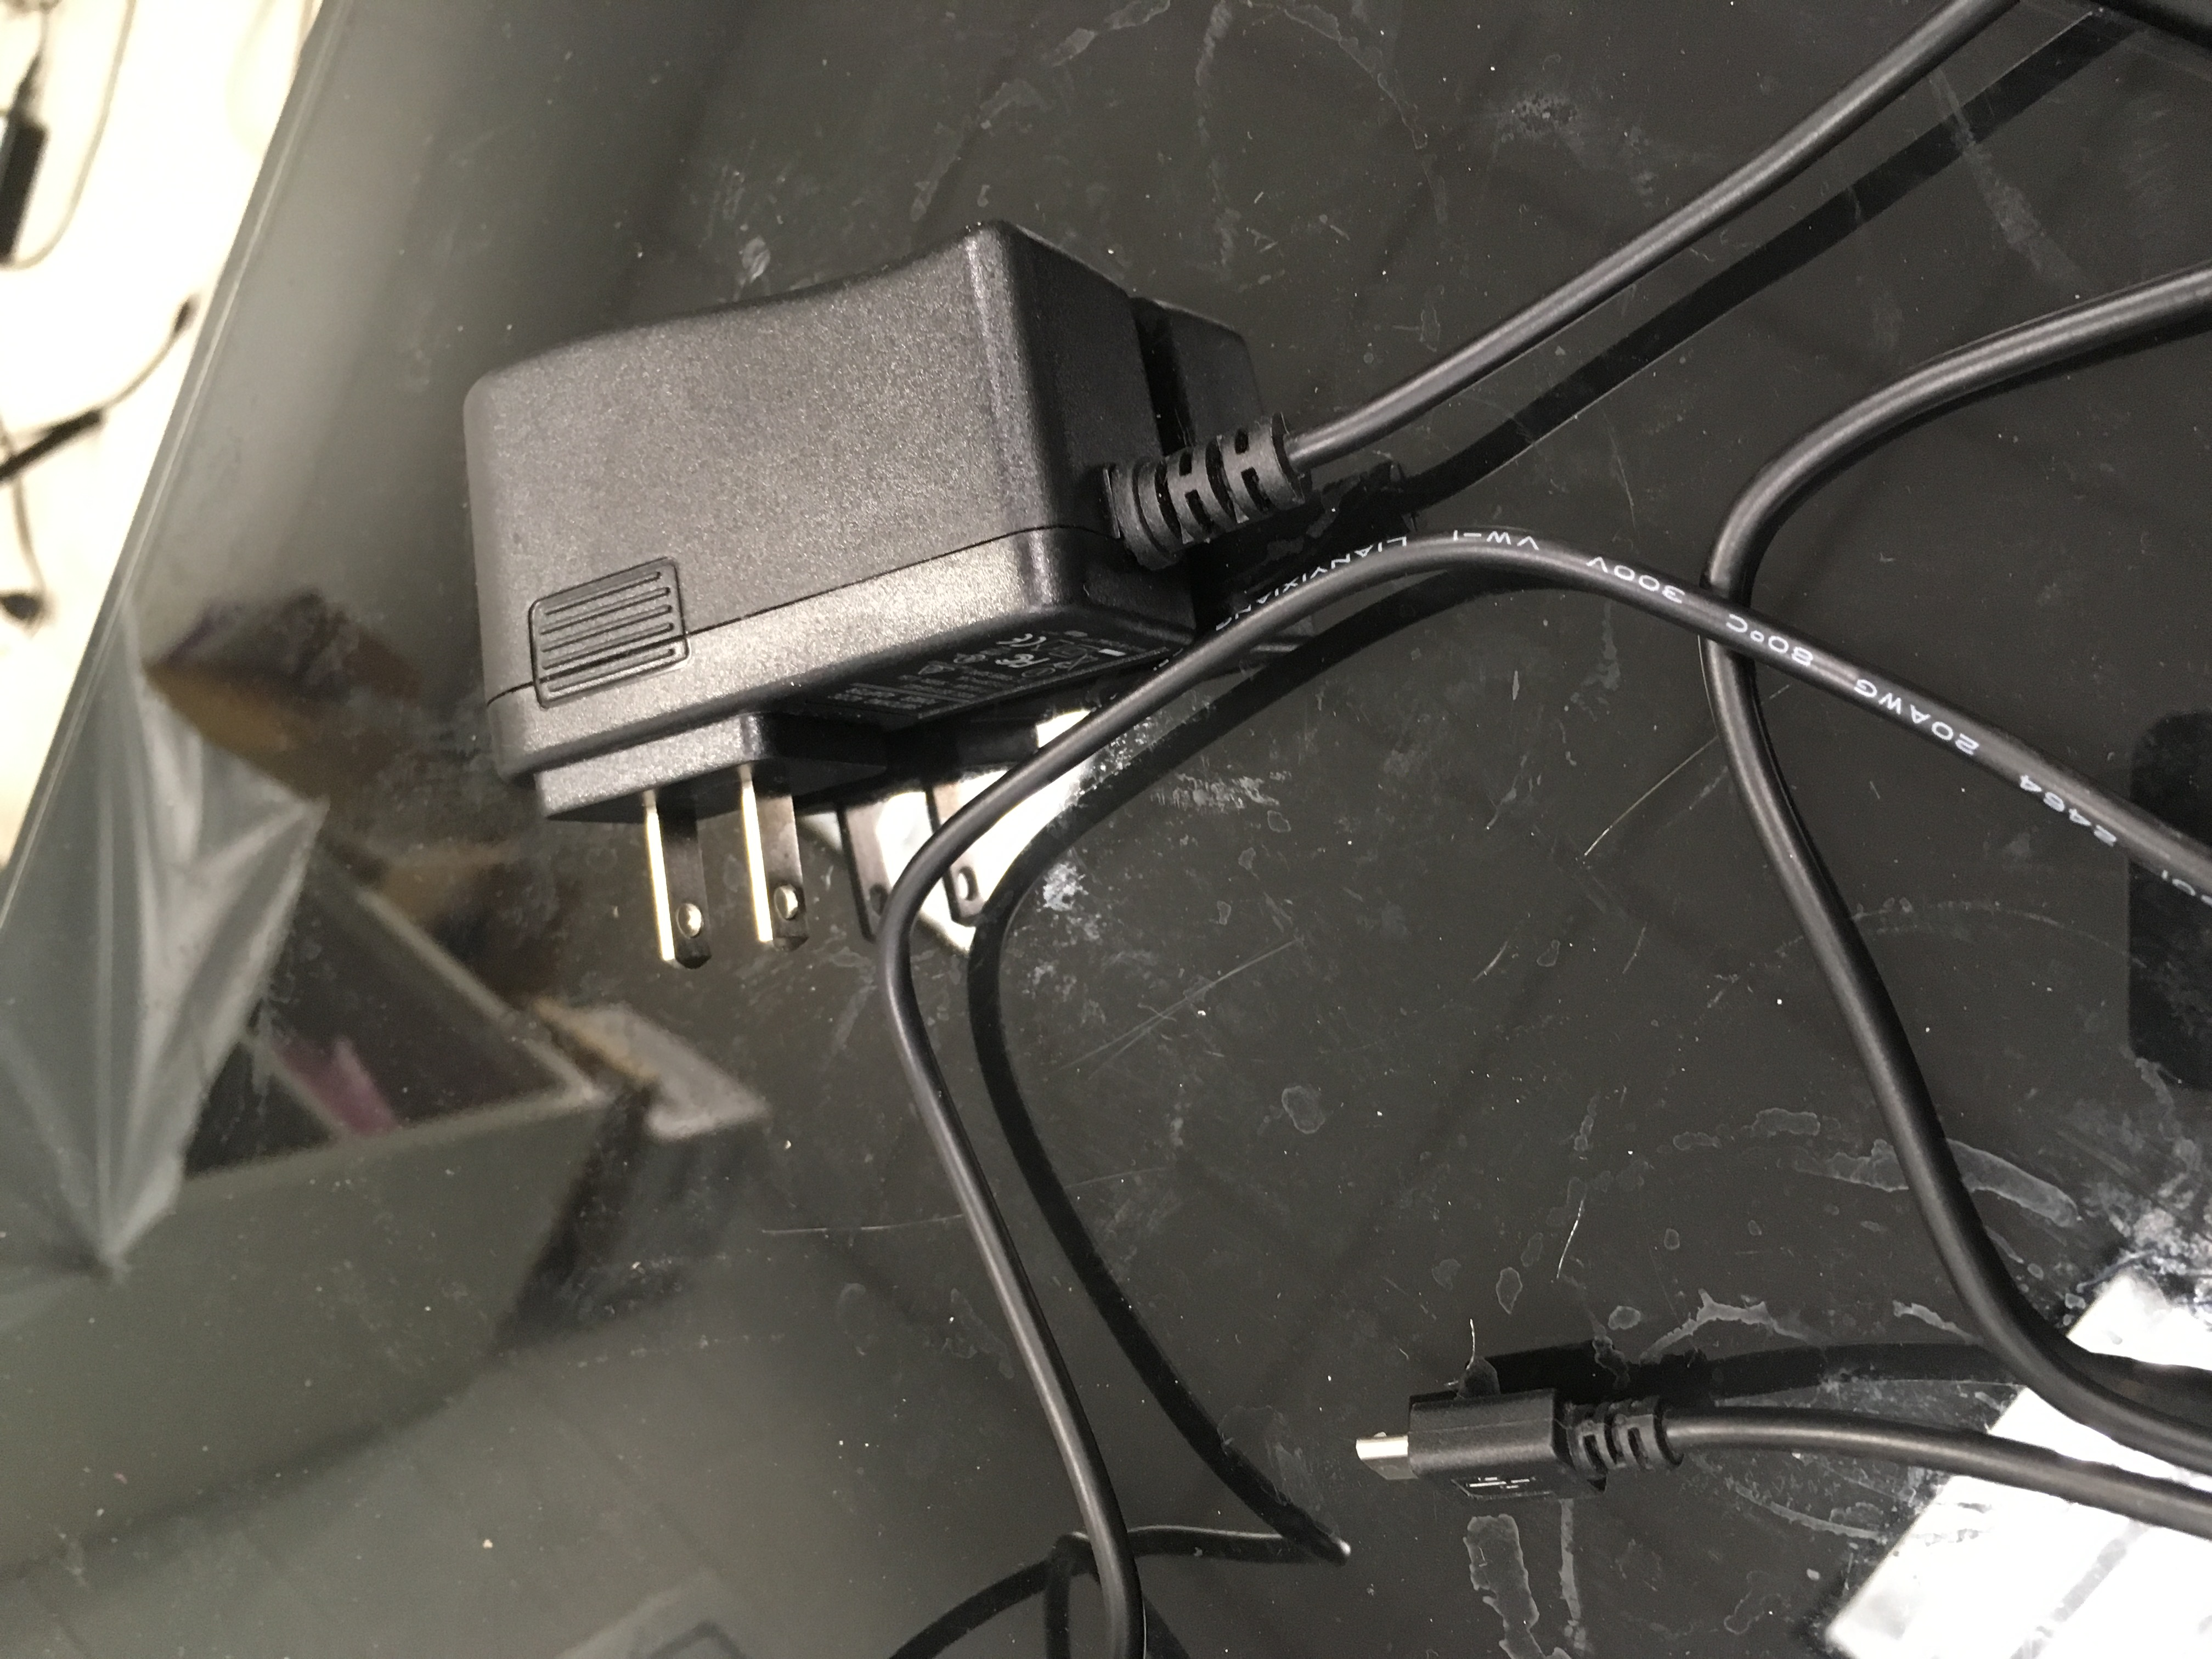
\includegraphics[angle=-90, width=\textwidth]{./figures//IMG_0710.JPG}
    \caption{Adapter 2}
    \label{fig:p2}
  \end{subfigure}
  \label{fig:pp}
\end{figure*}

\end{document}
